\section{State of the Art}

\subsection{On Affordances}

\subsubsection{The Concept of Affordances in HCI}

In Human-Computer Interaction, the term "affordance" is essential for understanding how users engage with interfaces, serving as a bridge between User Interface (UI) design and User Experience (UX).
Affordances refer to the properties or characteristics of an object (or digital element) that suggest its possible uses, guiding users toward intended actions within an interface.

The concept originated with Gibson (1977) \cite{gibson1977theory}, who introduced affordances in the context of ecological psychology.
For Gibson, affordances are action possibilities inherent in an environment that exist regardless of whether an actor perceives them.
For example, a chair affords sitting regardless of whether someone realizes it or uses it for that purpose.
This perspective highlights that affordances are rooted in the functional capabilities of an environment or object.

Building upon Gibson's foundational work, Norman (1988) \cite{norman1988psychology} adapted the concept to HCI, emphasizing how affordances in interfaces provide cues about possible interactions.
Norman expanded the idea to focus on perceived affordances, explaining that objects or interface elements should offer visual hints that communicate how they can be used.
For instance, a button's design may indicate that it is clickable, through shading, placement, or other visual markers, signaling users toward the appropriate interaction without explicit instructions.
Norman’s interpretation underscores the role of perception in usability: an affordance is effective in HCI when it is both present and easily recognizable.

This refinement of affordances into perceived cues is integral to user experience design, as it shapes how easily and intuitively users navigate an interface.
Clear affordances reduce cognitive load, allowing users to engage with minimal friction, leading to a seamless, satisfying UX.
By leveraging users' existing mental models, affordances can guide interactions effectively.
For instance, a trash can icon is widely recognized as affording deletion—a shared metaphor that aids usability.

\begin{figure}[!h]
    \centering
    
\includegraphics[width=\textwidth/3]{iconsAffordances.png}
    \caption{Functional icons indicate actions.}
    \vspace{0.1cm}
    \label{fig:affordances}
\end{figure}

Affordances in HCI enhance both functionality and understandability, forming a bridge between the UI elements users interact with and the UX that shapes their experience.
The more intuitive and apparent these affordances, the more effortlessly users can navigate and feel in control of the interface, optimizing overall interaction.

\subsubsection{Building on Affordances}

In the previous section, we explored the concept of affordances as a fundamental link between User Interface (UI) and User Experience (UX).
Affordances guide users through an interface by providing signals about the possibilities an action can unlock\cite{10.20380/gi2000.24}\cite{10.1177/1086026618803729}.
When these affordances are clear, users can intuitively understand what actions are possible.
However, as digital interfaces evolve, particularly in the realms of augmented reality (AR) and artificial intelligence (AI), we encounter new types of interfaces where affordances are less explicit.
These \textbf{low-signaling, high-possibility} systems challenge traditional UI and UX paradigms, introducing new complexities in how users navigate and interact with the possibilities afforded by these systems.

\subsubsection{ Low Signaling, High Possibility Interfaces}

Low-signaling, high-possibility interfaces are designed with minimal explicit cues, offering limited guidance on potential interactions while enabling a broad scope of possible outcomes.
These interfaces challenge traditional human-computer interaction frameworks, as they minimize explicit affordances, making it difficult for users to grasp the system's full functionality.
This limited signaling can create a perceptual gap, wherein the extensive potential of the interface may not align with the user's ability to easily interpret or interact with it, creating friction in usability and discovery processes.

In this context, the affordances competition hypothesis \cite{cisek2010neural}, offers insights into understanding how users navigate such interfaces.
According to this hypothesis, interactive behaviors rely on simultaneous processes in which potential actions are specified and selected in real-time rather than in serial stages.
This framework contrasts with traditional cognitive models, suggesting that users may not process low-signaling interfaces through linear steps but instead perceive and select actions dynamically, aligning more closely with real-time interactive systems that emphasize immediacy and fluidity in human-computer interactions.
Thus, low-signaling interfaces may require users to engage in this kind of affordance competition, evaluating and selecting options in parallel rather than relying on pre-defined instructions.

Moreover, research on HCI design principles underscores the importance of aligning system functionality with users' mental models to enhance overall usability and satisfaction \cite{10.1051/e3sconf/202339904037}.
Interactive systems that complement human cognitive processes and intuitively support the user's decision-making foster a more accessible and fulfilling experience.
In low-signaling interfaces, however, this alignment becomes challenging due to the minimal cues provided, emphasizing the need for adaptive and responsive design elements that aid users in discovering the high-possibility actions available.
Consequently, achieving a balanced design in these interfaces requires understanding human cognition and designing responsive elements that can subtly guide user interaction without overwhelming or reducing the interface’s inherent flexibility.

\subsubsection{ Signaling Levels vs. Possibility Levels}

To effectively design for both usability and richness in interaction, it's important to understand the balance between signaling levels and possibility levels:

\begin{itemize}
    \item \textbf{High Signaling, Low Possibility:} These interfaces are straightforward and easy to use, offering clear affordances for a limited range of actions. For instance, a simple media player might feature a play/pause button, volume controls, and a slider for adjusting the timeline—each with an obvious function.
    \item \textbf{Low Signaling, High Possibility:} These interfaces, by contrast, are complex, offering numerous interaction possibilities, but with minimal guidance or affordances. Voice command systems or gesture-based interfaces often fall into this category, where the user must experiment or learn to discover the breadth of possible interactions.
\end{itemize}
    


In many cases, increasing signaling—through visual or other sensory affordances—enhances the user's ability to explore the full potential of a system.
However, increasing signaling can clutter the user's experience and overwhelm the interface, limiting the immersion and fluidity.

\subsubsection{ Augmented Reality \& Signaling Challenges}

Augmented Reality (AR) exemplifies the unique challenges of designing low-signaling, high-possibility interfaces\cite{10.1145/2254556.2254569}.
In AR, users can interact with digital elements seamlessly integrated into their physical surroundings, creating opportunities to blend the virtual and real.
However, signaling these interactions can be difficult, as too many visual cues may diminish the immersive experience, disrupting the cohesion between digital overlays and physical space.

An AR interface may offer rich interaction possibilities, such as manipulating virtual objects, triggering animations, or accessing information through gestures, voice commands, or interactions with physical items.
However, without intuitive affordances—like context-aware hints, subtle animations, or gestures that intuitively link to real-world actions—users may struggle to understand the interface’s potential.
The vast range of interactions that AR enables is thus limited by how effectively these options are communicated.

Furthermore, AR introduces a unique third-person challenge: a person without AR gear cannot readily interpret the interactions between AR users and digital elements, leading to an exclusionary effect in shared physical spaces.
This highlights the need for AR interfaces to create inclusivity by making interactions more accessible and understandable even to those without AR devices.
Integrating AR elements into the physical environment through clear, minimalistic cues—such as small indicators or interactive physical anchors—can help bridge this gap, allowing both AR-equipped and non-equipped participants to follow the interaction flow.

To achieve intuitiveness and fluidity, AR interfaces should minimize the learning curve and reduce the need for elaborate tutorials.
The goal is to make interactions so intuitive that users can understand and engage with AR environments effortlessly, enhancing both user experience and accessibility.
Ultimately, the goal of AR interfaces should be to achieve intuitiveness and fluidity, reducing the need for a steep learning curve or extensive tutorials.
Effective AR affordances should allow users to explore and engage with the environment naturally, discovering interactions as they would in the physical world.
By prioritizing intuitive, fluid interactions, AR interfaces can empower users to fully leverage the technology’s potential with minimal guidance, enhancing both usability and user experience.

\subsubsection{ AI Enabled High-Possibility, Low-Signaling Interfaces}

Artificial Intelligence serves as a crucial enabler for low-signaling, high-possibility interfaces\cite{neches1986intelligence}.
By interpreting user intent and providing contextual cues, AI enhances intuitive interaction in environments where explicit visual affordances are limited\cite{9820378}.
Through real-time analysis of user behavior and context, AI-driven systems can offer subtle, adaptive guidance, creating an experience that feels natural and minimally intrusive.

For instance, in low-signaling interfaces such as voice assistants, AI interprets natural language inputs, eliminating the need for traditional visual cues.
This approach simplifies interactions, allowing users to engage seamlessly without explicit prompts.
Similarly, in Augmented Reality environments, AI can track a user’s gaze, gestures, or position in real-time, delivering just-in-time affordances that guide the user without disrupting immersion.
By responding dynamically to user actions, AI transforms the interface into a fluid, context-sensitive experience, enabling users to explore the system’s capabilities without facing a steep learning curve or being overwhelmed by signals.

AI also addresses the "high-possibility" aspect of these interfaces by unlocking functionalities that would otherwise be inaccessible.
Generative AI, for example, facilitates complex tasks like on-the-fly image creation, code generation, or data synthesis, all of which expand the potential actions available within an interface.
In creative tools, this enables users to generate images, design interactive elements, or even produce code using simple, high-level commands.
Through capabilities like generative AI, systems gain a wide range of possible interactions without requiring a corresponding increase in explicit controls, allowing users to accomplish complex tasks with minimal input.

\subsubsection{ AR and AI: A Symbiotic relationship}

The convergence of Artificial Intelligence and Augmented Reality creates a powerful synergy that addresses the inherent challenges of low-signaling, high-possibility interfaces in AR environments.
While AR offers a high degree of interaction potential by blending digital elements with physical surroundings, it is often limited by the difficulty of signaling these possibilities in an intuitive, immersive manner.
AI, on the other hand, enables adaptive affordances, capable of interpreting user intent and dynamically generating cues, effectively bridging this gap.

In AR, the complexity of potential interactions—such as manipulating virtual objects, accessing hidden layers of information, or collaborating with others—is constrained by the system's ability to guide users effectively without overwhelming visual indicators.
Here, AI proves invaluable.
By analyzing gestures, gaze, and contextual factors in real time, AI can offer subtle prompts, adjust visual affordances, or predict actions, thus empowering users to explore and interact with AR content fluidly.
For example, if a user’s gaze lingers on a virtual object, AI could provide a discreet visual cue, indicating that the object is interactive, without detracting from the overall immersive experience.

Moreover, AI's generative capabilities elevate AR to a new level of high-possibility interaction.
Generative AI models can dynamically create content such as images, textures, or even functional code within the AR environment, broadening the scope of what users can accomplish.
This expands AR from a static interface to an evolving, interactive canvas where users are limited only by their imagination rather than interface constraints.
By enabling such high-possibility functionalities, AI transforms AR from a fixed display of virtual elements to a responsive, co-creative environment.

Together, AI and AR cultivate a low-signaling, high-possibility interface that enhances user experience through intuitiveness and adaptability.
AI alleviates the signaling limitations of AR by dynamically responding to user intent, while AR provides a tangible canvas for AI-driven possibilities, blending digital and physical realms.
This symbiotic relationship ultimately fosters an accessible, immersive environment, where users can interact freely and creatively, with minimal guidance and maximal opportunity.

\subsection{ Interpreting user actions in AR}

Tracking user movements in AR is challenging due to the need for real-time accuracy, low latency, and efficient processing on mobile devices.
These requirements are complicated by factors like variable lighting, fast motions, and limited device resources, all of which demand highly optimized algorithms and adaptive processing to deliver smooth, immersive interactions.

\begin{figure}[!h]
    \centering
    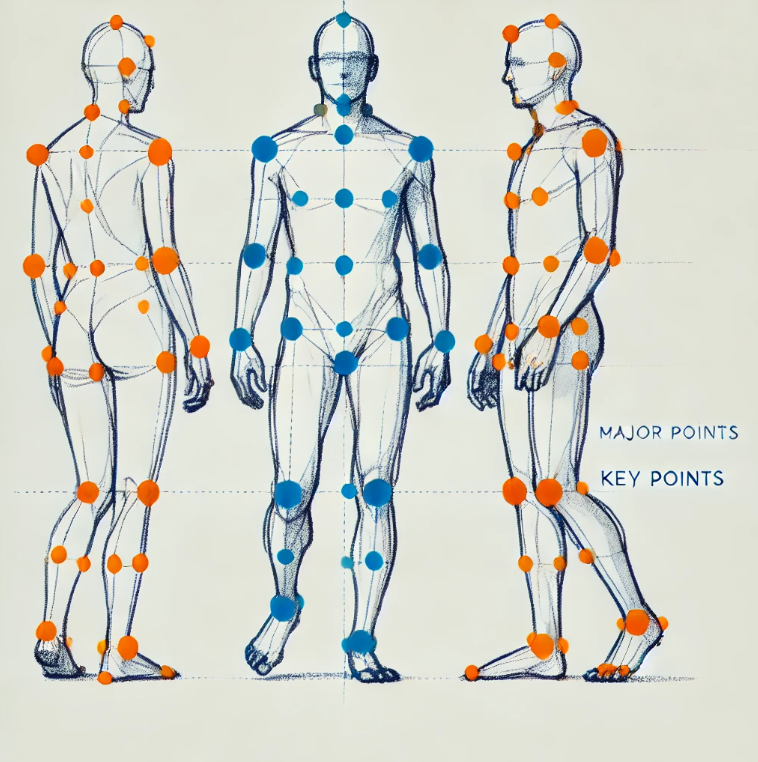
\includegraphics[width=\textwidth/3]{mediapipeKP.png}
    \caption{Simplified sketch showcasing keypoint tracking.}
    \vspace{0.1cm}
    \label{fig:kptracking}
\end{figure}

\subsubsection{Overview of MediaPipe for Edge Devices in AR}

MediaPipe\cite{lugaresi2019mediapipe} is a powerful framework for enabling high-fidelity body pose estimation on edge devices.
This framework uses a pipeline to detect and track human poses in real time, which has expanded the possibilities for AR applications by allowing overlay interactions that are responsive, intuitive, and suitable for everyday mobile devices.
MediaPipe's flexibility allows it to run on mobile devices, desktops, and even in web environments, ensuring accessibility for diverse applications such as fitness tracking, dance, sign language recognition, and full-body gesture control.

\begin{figure}[!h]
    \centering
    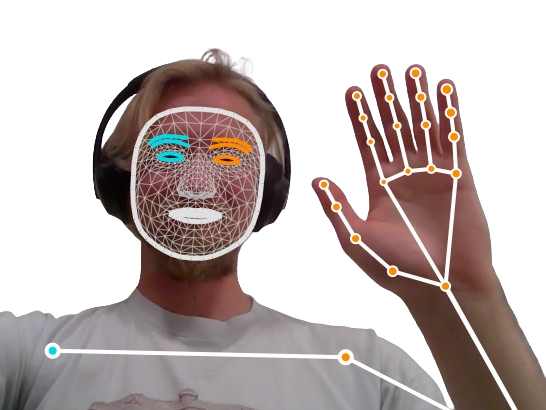
\includegraphics[width=\textwidth/2]{mediapipe.png}
    \caption{Key points tracked by mediapipe.}
    \vspace{0.1cm}
    \label{fig:mediapipe}
\end{figure}

In AR applications, MediaPipe Pose facilitates the seamless integration of digital content with physical movements.
With its ability to infer 33 3D landmarks and a background segmentation mask in real time, MediaPipe provides accurate body pose tracking that supports real-world overlays.
This makes it an ideal solution for applications that require responsiveness and precision, such as interactive exercise tutorials, real-time motion-based games, or immersive social experiences through virtual avatars.
By delivering such features on lightweight devices, MediaPipe enables more inclusive and accessible AR solutions, broadening AR’s reach into consumer-ready devices like smartphones and AR glasses.

\subsubsection{Comparison with other Frameworks}

While frameworks like OpenPose\cite{cao2017realtime} have demonstrated high accuracy in pose tracking, they often depend on powerful desktop environments for processing.
MediaPipe’s edge lies in its ability to deliver real-time pose estimation on mobile and web platforms, specifically optimized to maintain high performance on devices with limited computational resources.

MediaPipe Pose, powered by BlazePose\cite{bazarevsky2020blazepose}, adopts a two-step detector-tracker ML pipeline. The detector identifies the person or pose’s region of interest (ROI) within the frame, while the tracker predicts pose landmarks and segmentation within this ROI. This approach minimizes computational load by selectively activating the detector only for the first frame or when the tracker loses sight of the pose, ensuring that subsequent frames can rely on the previously identified ROI.
This contrasts with frameworks like AlphaPose and Apple Vision, which typically employ continuous processing, potentially consuming more resources and leading to latency issues on mobile devices.
\begin{figure}[!h]
    \centering
    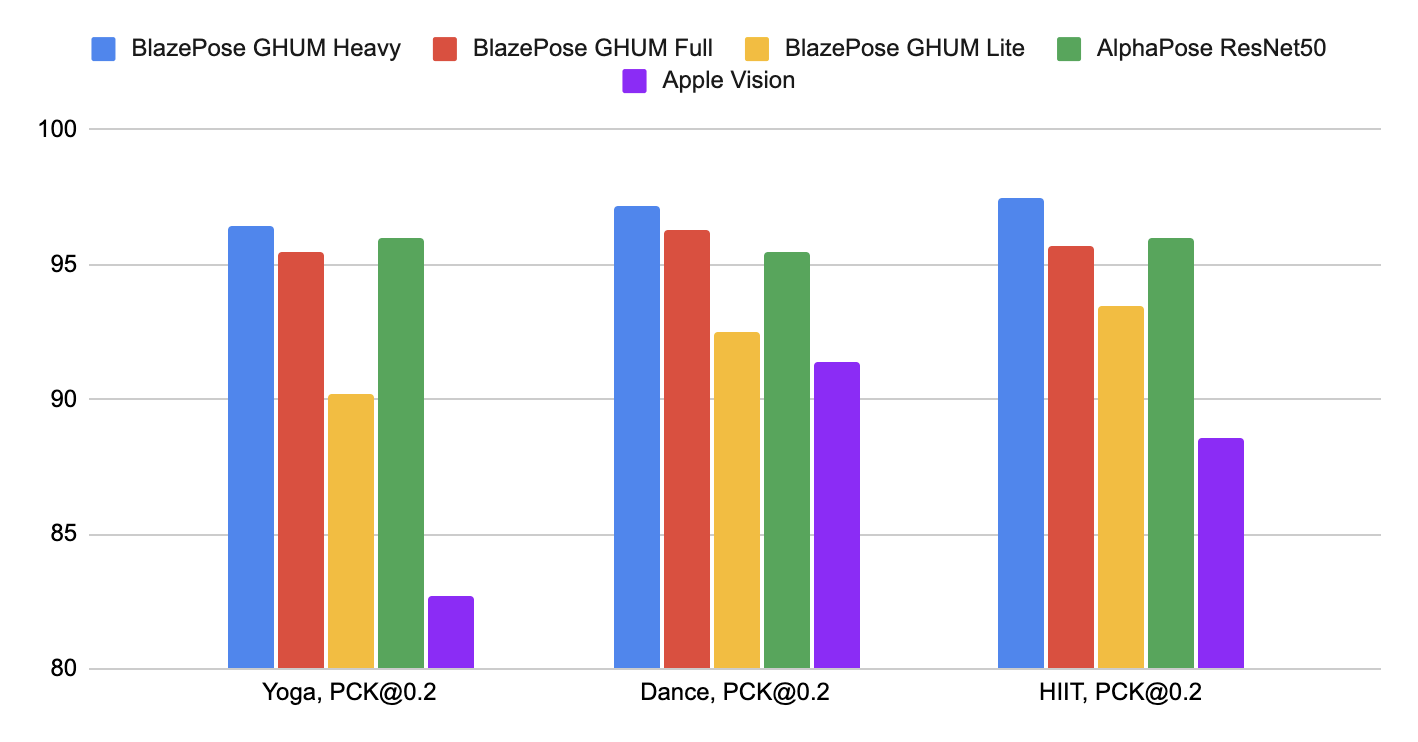
\includegraphics[width=\textwidth]{arFrameworkComp.png}
    \caption{Quality evaluation of different Frameworks on the PCK@0.2 Benchmark.}
    \vspace{0.1cm}
    \label{fig:arFrameworks}
\end{figure}
Moreover, MediaPipe’s holistic pipeline allows it to integrate multiple tasks—pose, face, and hand tracking—into one efficient graph, which is a significant differentiator from solutions requiring individual modules for each task.
Benchmarks also demonstrate that MediaPipe’s models, like BlazePose GHUM Lite, can achieve 20ms latency on mobile devices, outperforming heavier models such as BlazePose GHUM Heavy and comparable alternatives from Apple Vision.
This efficiency not only allows real-time tracking across various AR contexts but also opens new possibilities for developing lightweight, scalable AR applications that can run smoothly even on lower-end devices.

\subsubsection{MediaPipe Holistic Architecture and Modular Design}

MediaPipe Holistic is a comprehensive framework that differentiates itself from standalone models like BlazePose by integrating pose, face, and hand tracking into a unified system.
This holistic approach offers a unique advantage for AR applications requiring real-time, multi-modal tracking across these three key body regions.
By tracking multiple modalities within a single framework, MediaPipe Holistic enables immersive and cohesive AR experiences, allowing interactions that rely on the synchronous tracking of head, hands, and body positions—essential for applications like gesture-based controls, sign language recognition, fitness analysis, and interactive AR effects.

To achieve this integration, MediaPipe Holistic relies on distinct models tailored to each tracking component (pose, face, and hands), optimized for high performance and low latency.
Each component operates independently but is semantically aligned through a multi-stage pipeline, which leverages the strength of each model while ensuring the output remains consistent across all regions. This pipeline begins by estimating the user’s full-body pose with BlazePose’s pose detector.
It then identifies regions of interest for each hand and the face, recropping the full-resolution input frame to improve accuracy before applying task-specific face and hand models.
The result is a cohesive set of 543 landmarks: 33 for the body, 468 for the face, and 21 for each hand, creating an accurate, detailed, and continuous tracking solution for AR applications.
\begin{figure}[!h]
    \centering
    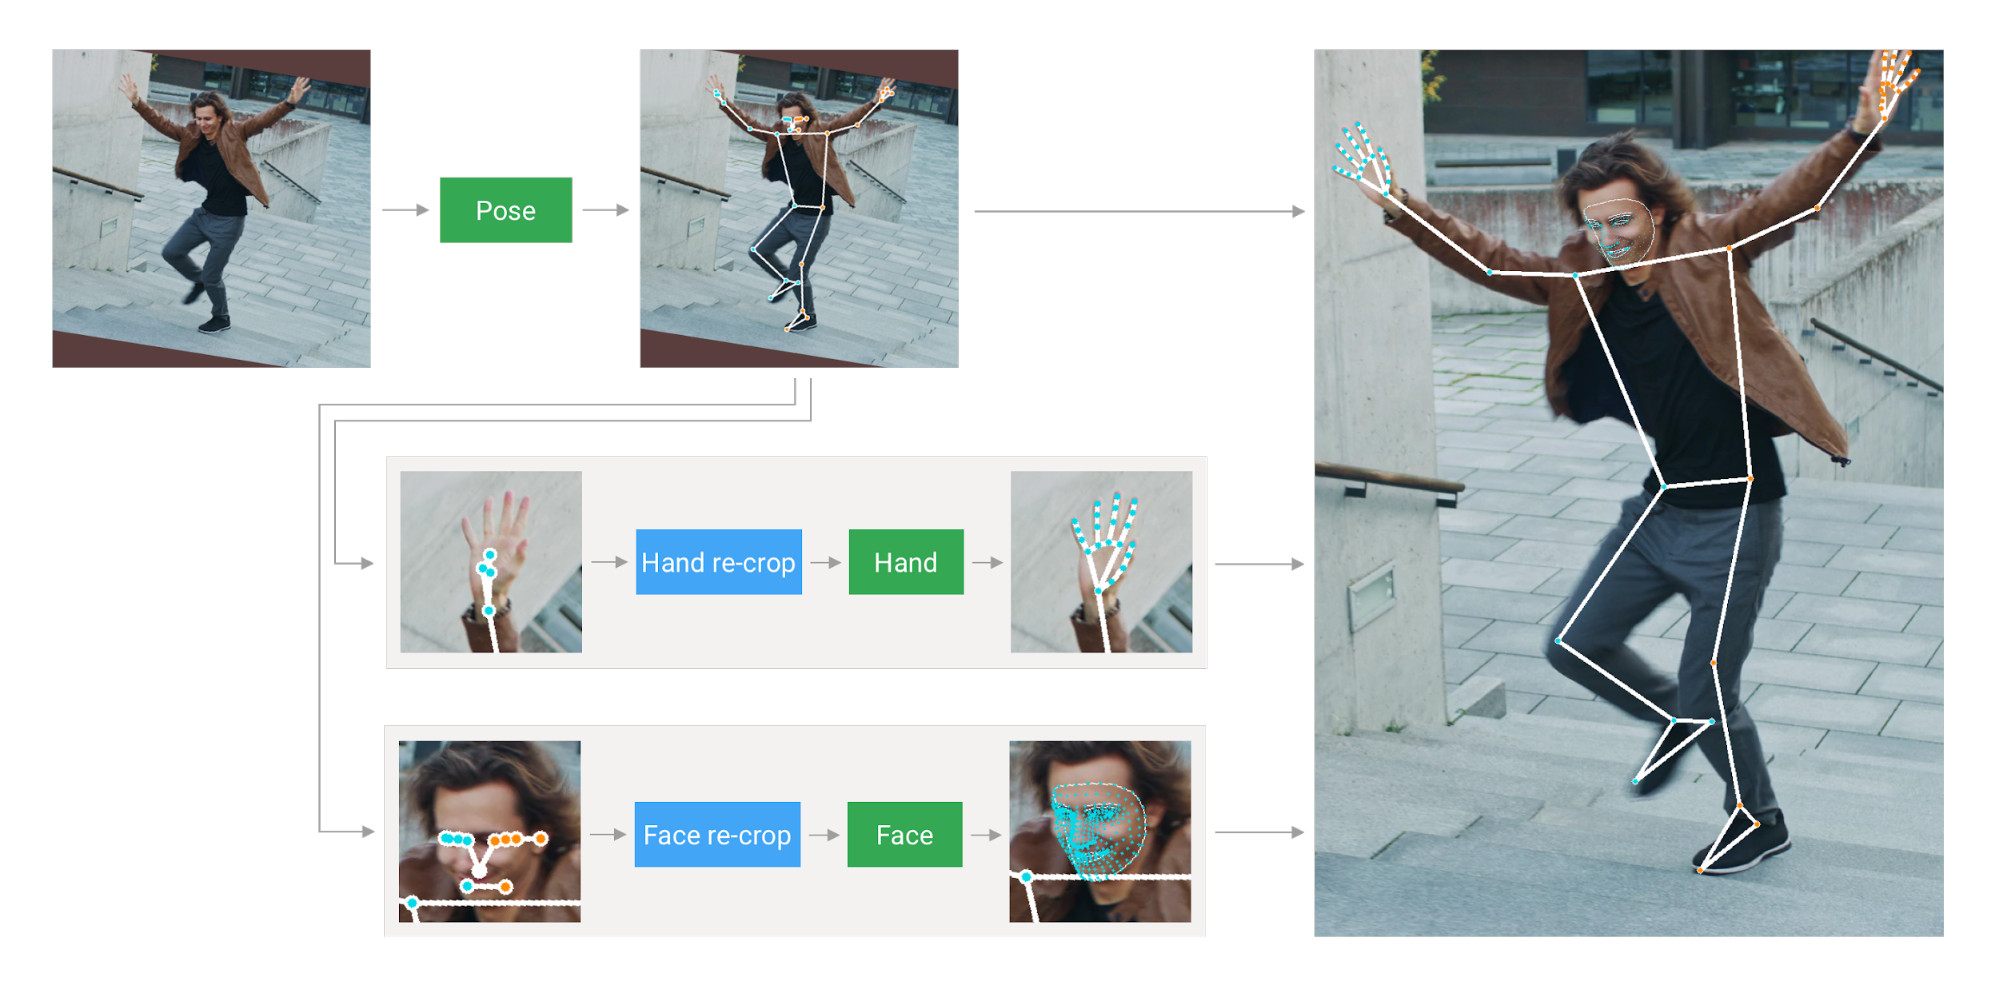
\includegraphics[width=\textwidth]{holistic.jpeg}
    \caption{Overview of the multi-stage pipeline in MediaPipe Holistic.}
    \vspace{0.1cm}
    \label{fig:holisticArchitecture}
\end{figure}

\subsubsection{Key Model Optimizations}


MediaPipe achieves exceptional performance on edge devices through a series of targeted optimizations, allowing it to deliver accurate, real-time tracking with minimal computational load.
These optimizations are critical for enabling MediaPipe to perform smoothly on mobile devices, making it ideal for AR applications that demand low latency and responsiveness.

\begin{itemize}
    \item \textbf{Graph-Based Pipeline for Efficient Processing:} At the core of MediaPipe's efficiency is its graph-based pipeline, a modular structure where each computational task, such as pose detection or face tracking, functions as an independent node within a directed graph.
    This setup allows tasks to run only when needed, reducing redundant computations and streamlining data flow through the pipeline.
    The graph-based design also enables parallel processing by assigning distinct tasks to separate CPU or GPU cores, maximizing hardware utilization.
    By leveraging this modular approach, MediaPipe efficiently manages real-time data flow, reducing latency and enhancing the responsiveness of AR interactions.

    \item \textbf{Lightweight and Quantized Model Architecture:} To balance accuracy and computational efficiency, MediaPipe’s models are carefully designed to reduce floating-point operations (FLOPs) and minimize parameter count.
    This lightweight architecture enables MediaPipe to perform complex inference tasks effectively even on resource-limited devices.
    Further optimization is achieved through quantization, converting 32-bit floating-point weights to 8-bit integers, which substantially reduces memory usage and accelerates processing times without compromising accuracy.
    This combination of a lightweight design and quantization enables MediaPipe to deliver real-time performance on mobile devices.

    \item \textbf{Adaptive Inference with Frame Skipping:} MediaPipe’s adaptive inference and frame-skipping techniques are essential for managing processing power effectively.
    By dynamically reducing processing for frames with minimal movement, MediaPipe optimizes resource usage, reducing battery drain while maintaining high responsiveness.
    In high-motion scenarios, the system seamlessly adjusts by resuming full-frame inference to ensure consistent performance.
    This flexibility allows MediaPipe to conserve resources during low-demand periods while maintaining the responsiveness needed for interactive AR applications.

    \item \textbf{Integrated Parallel Processing:} MediaPipe takes advantage of the multicore architecture in modern mobile devices, enabling simultaneous processing across pose, hand, and face tracking components.
    By distributing these tasks across available CPU or GPU cores, MediaPipe achieves real-time, synchronized multi-modal tracking without overloading the device’s resources.
    This parallel processing capability is particularly valuable in AR applications where coordinated tracking of multiple regions—such as body, face, and hands—enables smooth, uninterrupted user interactions.
\end{itemize}


\subsubsection{Conclusion}

MediaPipe stands as a pioneering framework for delivering real-time, high-fidelity tracking across multiple modalities on edge devices, making it an ideal solution for AR applications.
Through a combination of modular graph-based architecture, adaptive inference techniques, and carefully optimized model designs, MediaPipe achieves a balance of accuracy and efficiency that enables it to run seamlessly even on resource-constrained devices.

The framework’s flexibility, from lightweight and quantized models to advanced data flow control and parallel processing capabilities, showcases its adaptability across a range of devices—from mobile phones to AR glasses.
MediaPipe’s holistic approach, which integrates body, face, and hand tracking within a unified system, opens the door to immersive, interactive experiences that push the boundaries of what’s possible on mobile platforms.
This adaptability not only supports a wide range of AR applications, such as fitness tracking, gesture-based controls, and social augmented reality, but also paves the way for future advancements in edge-based computing and user interaction.

\subsection{ The Evolution of Natural Language Processing}

\subsubsection{ From N-Grams to Modern LLMs}

Natural Language Processing (NLP) has undergone a remarkable evolution in the field of machine learning, from early techniques like N-grams \cite{Mar13} to the advent of modern large language models (LLMs).
Each milestone in this progression reflects the increasing complexity of language understanding and the growing sophistication of computational models designed to process human language.
Today, LLMs are not just powerful language processors; they have become semantic operators, revolutionizing how we interpret and interact with language.
This section explores the evolution of NLP, highlights the rise of LLMs as semantic operators, and explains how these models are reshaping Human-Computer Interaction by enabling interfaces with low affordance through low signaling and high possibility.

\subsubsection{N-Grams and Statistical Models}

In the early stages of NLP, statistical models like \textbf{N-grams} were used to predict the likelihood of word sequences.
N-grams operate on the probability of a word occurring based on the preceding N-1 words.
For example, a bigram model predicts a word based on the one word before it, while a trigram model uses the two preceding words.
Though simple, N-grams were effective in various applications, such as speech recognition and text generation, offering a straightforward way to model language by counting occurrences and calculating probabilities.

One notable application of N-grams was in early predictive text systems, like the original iPhone keyboard\cite{kocienda2018creative}.
With its small on-screen keys, the iPhone relied on character-level n-grams to help users type accurately by predicting likely next letters and correcting common typos.
By understanding the statistical likelihood of certain letter combinations, the keyboard could infer users' intended words, even when their finger presses were imprecise.
Although limited in scope, these early models significantly improved typing accuracy on a touchscreen, illustrating how statistical NLP techniques laid the foundation for practical applications in HCI.

However, these models had significant limitations, especially regarding broader context in language. N-grams could only account for short-range dependencies, making them prone to errors when handling ambiguity or meaning, as they were purely statistical and lacked a deeper semantic understanding.
The reliance on limited context highlighted the need for more advanced methods, eventually leading to NLP models that could better capture the complexities of human language.

\subsubsection{ Neural Networks and Word Embeddings}

The next significant leap in NLP came with the introduction of \textbf{neural networks} and \textbf{word embeddings}, particularly through models like Word2Vec \cite{rong2014word2vec} and GloVe\cite{pennington2014glove}.
Word embeddings transformed how machines interpreted language by mapping words to dense vectors that captured semantic relationships. This allowed words with similar meanings to have similar vector representations, enabling models to understand relationships like "king" is to "queen" as "man" is to "woman."

\begin{figure}[!h]
    \centering
    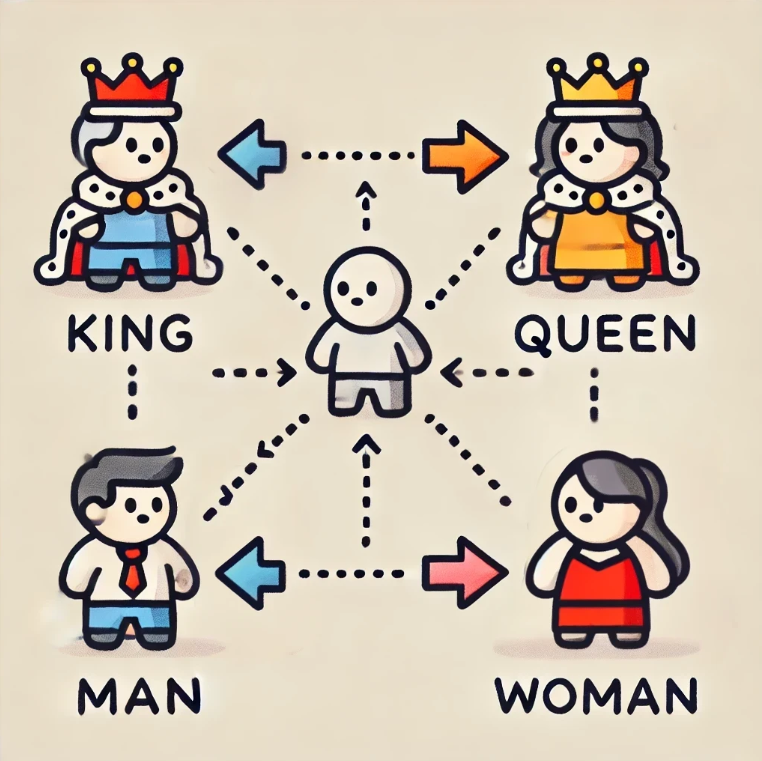
\includegraphics[width=\textwidth/3]{embedding.png}
    \caption{The mathematical operation that transforms the embedding of "man" to "woman" also transforms the embedding of "king" to "queen".}
    \vspace{0.1cm}
    \label{fig:embeddings}
\end{figure}

These embeddings, while a major step forward, still struggled with polysemy (words having multiple meanings) and couldn’t handle long-range dependencies well.
The need for a model that could understand context over entire sentences or paragraphs led to the development of \textbf{recurrent neural networks (RNNs)} \cite{Rumelhart1986LearningIR} and \textbf{long short-term memory (LSTM)} \cite{hochreiter1997long} networks, which improved the ability to capture sequential dependencies in language.

\subsubsection{ The Transformer Era and Large Language Models}

The breakthrough that brought NLP into the modern era was the development of the \textbf{Transformer} architecture, first introduced in the "Attention is All You Need" paper by Vaswani et al. in 2017 \cite{vaswani2017attention}. Unlike RNNs, Transformers rely entirely on a self-attention mechanism, allowing the model to focus on different parts of a sentence simultaneously, regardless of their position.
This enabled better handling of long-range dependencies and opened the door for scaling NLP models to unprecedented levels.

\begin{figure}[!h]
    \centering
    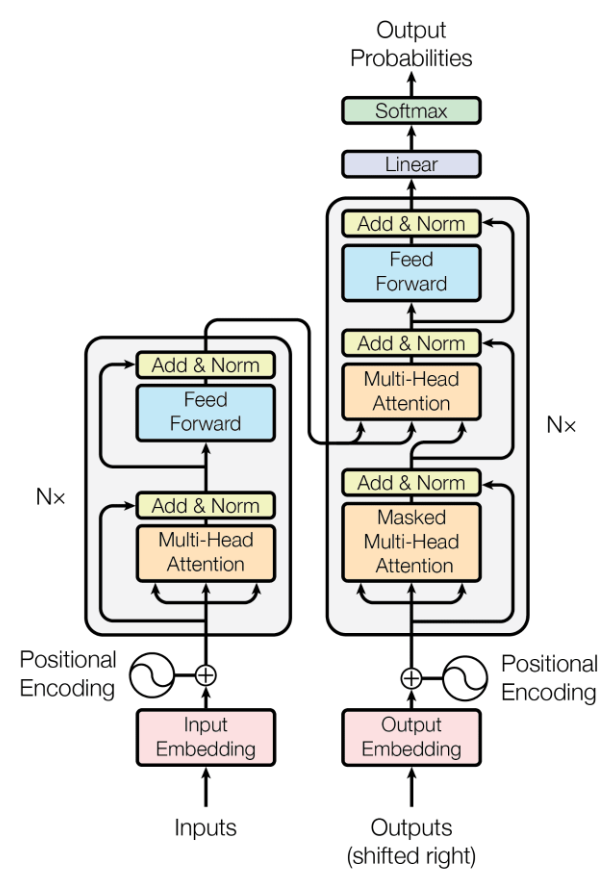
\includegraphics[width=\textwidth/2]{trasnformer.png}
    \caption{Overview of the Transformer architecture.}
    \vspace{0.1cm}
    \label{fig:transformer}
\end{figure}

Building on the Transformer architecture, \textbf{large language models (LLMs)} like \textbf{GPT (Generative Pre-trained Transformer)}\cite{radford2018improving} and \textbf{BERT (Bidirectional Encoder Representations from Transformers)}\cite{devlin2018bert} revolutionized NLP. LLMs trained on vast corpora of text have demonstrated the ability to perform tasks such as text generation, translation, summarization, and even answering complex questions.
These models don’t just analyze words—they understand context, intent, and meaning on a deep level, making them far more adept at processing human language.

The rise of Large Language Models (LLMs) marks a significant shift in accessibility and democratization of deep learning technologies.
Historically, large deep learning models required extensive computational resources and were primarily accessible to those with the expertise to manage complex architectures.
However, the introduction of \textbf{pay-as-you-go APIs} like ChatGPT and Claude, alongside open-source platforms like \textbf{Hugging Face}, has drastically lowered the barriers to entry.
These services enable developers to access and integrate powerful LLMs without the need for specialized infrastructure or deep expertise.
Now, even a simple microcontroller or edge device can leverage web APIs to tap into cutting-edge NLP capabilities, significantly reducing both development and maintenance costs.
This democratization has expanded the use of deep learning technologies, making them accessible to a broader audience across industries and enabling more innovation in human-computer interaction.

\subsubsection{ LLMs as Semantic Operators}

% One of the most powerful aspects of modern LLMs is their function as \textbf{semantic operators}.
% In computing, we are familiar with mathematical and logical operators, which are hardware-friendly and easily implemented.
% However, \textbf{semantic operators}, which deal with meaning and interpretation, were traditionally reserved for the human domain.
% With LLMs, machines can now function as semantic operators, interpreting, manipulating, and generating language in ways that reflect deeper understanding.

% For example, when presented with the sentence "The cat sat on the mat," a mathematical model would simply process the syntax.
% However, an LLM can infer more—understanding that "cat" is an animal, "sat" refers to the action of sitting, and "mat" is a surface.
% More complex interpretations, like summarizing a paragraph or making inferences based on context, were historically exclusive to human cognition but are now within the domain of LLMs.

% The ability of LLMs to act as semantic operators enables machines to comprehend and engage with the subtleties of language, making them invaluable for natural language tasks in HCI.
% They allow systems to interact more naturally with users by understanding the meaning behind queries, interpreting ambiguous input, and even generating responses that align with human expectations.

Modern LLMs have introduced a groundbreaking capability in computing: acting as semantic operators.
While traditional computing relies on mathematical and logical operators—mechanisms well-suited to hardware implementation—semantic operators handle meaning and context, areas previously limited to human cognition.
With LLMs, machines are now capable of interpreting, processing, and generating nuanced language, taking on a role that involves understanding rather than mere data processing.

The Sparks of AGI paper\cite{bubeck2023sparks} highlights that models like GPT-4 exhibit skills close to human-level performance across diverse domains, from mathematics to law, without needing tailored instructions.
This capacity is demonstrated through zero-shot prompting\cite{li2023practical}, where the model can perform a task based solely on general context, without examples.
For instance, a zero-shot prompt might be as simple as asking, "Summarize this paragraph," after presenting the model with a passage.
Despite the lack of detailed instructions, the model generates a concise summary by relying on its inherent understanding of summarization.
This zero-shot capability reveals the model’s ability to generalize knowledge across tasks, positioning it as an early form of artificial general intelligence (AGI).

Another powerful technique, few-shot prompting\cite{brown2020language}, allows LLMs to refine their responses by providing a small set of examples before asking the model to complete a similar task.
In the context of Human-Computer Interaction, few-shot prompting can be used to guide the model’s behavior in interpreting high-level commands.
For example, the LLM Whiteboard might prompt the model with a few examples like:

\begin{itemize}
    \item “Generate a bouncing ball animation in p5.js." -> associated reference code
    \item “Create a grid of circles that changes color every second." -> associated reference code
    \item “Draw a moving wave pattern." -> associated reference code
\end{itemize}

After these examples, the model is then asked to generate a new animation, such as “Create a rotating star shape,” with the expectation that it will follow the established style and coding framework.
This few-shot prompting technique primes the model to understand the format, purpose, and complexity expected in user commands, thereby improving the consistency and relevance of its responses.
By leveraging a small number of examples, few-shot prompting helps the model align closely with user intent and respond with greater accuracy in interactive systems.

Together, zero-shot and few-shot prompting highlight the versatility of LLMs as semantic operators, allowing them to bridge the gap between user intent and machine interpretation in a seamless, adaptable way.
By handling ambiguous language, responding contextually, and dynamically adapting to user needs, these prompting methods enable more natural and responsive AI-driven interactions.
This capability transforms LLMs from simple data processors into sophisticated collaborators.

% \subsubsection{ Semantic Operators and Their Role in HCI}

% In Human-Computer Interaction, semantic operators such as large language models are transforming how users interact with complex systems, especially within the framework of low-signaling, high-possibility affordances.
% As semantic operators, LLMs excel at interpreting context, predicting user intent, and generating responses that align with the user’s high-level goals, even when the interface offers few visual signals.
% The ability to support rich interaction with low signaling creates a flexible, high-possibility interface that aligns closely with natural human communication patterns.

% This interpretative power is particularly valuable in emerging technologies like augmented reality and AI-driven interfaces, where explicit affordances may be limited by the nature of the physical-digital blend.
% In these contexts, LLMs serve as the underlying layer that interprets user commands, allowing interaction through natural language or gestures without relying on predefined commands or extensive visual guidance.

% \subsubsection{ Conclusion }

% The progression of natural language processing, from early N-gram models to large language models, has fundamentally reshaped human-computer interaction by enabling machines to interpret, adapt, and respond to nuanced human language.
% In particular, LLMs, with their capacity to act as semantic operators, have proven essential in creating low-signaling, high-possibility interfaces—interfaces that minimize visual affordances while maximizing the range of potential actions and outcomes available to the user.
% This dynamic is especially effective in augmented reality, where LLM-driven interfaces empower users to interact intuitively through high-level instructions rather than explicit, screen-bound cues.

% For example, in an AR environment, a user might simply ask, "Show me the nearest restaurant," and the system, guided by an LLM, can accurately interpret the intent and context to provide relevant, actionable information without the need for extensive visual prompts.
% This illustrates how LLMs seamlessly bridge the gap between low-signaling and high-possibility interfaces, making complex systems more accessible and natural to use.
% As LLMs continue to advance, their impact on human-computer interaction will deepen, unlocking more seamless, intelligent, and context-aware interactions that align with human intent and extend the capabilities of natural language interfaces.

\subsubsection{ Semantic Operators and their Role in HCI}

In Human-Computer Interaction, semantic operators are transforming how users engage with complex systems.
The interpretative capacity of LLMs, allows them to act as "sounding boards", helping users ideate, refine, and evolve their thoughts rather than merely completing tasks\cite{Chen2023LargeLM}.
The interaction fosters a collaborative environment where human and AI capabilities complement one another, enhancing the user’s ability to generate nuanced and high-quality outputs.

Recent research highlights both the benefits and challenges of this collaboration, especially in creative contexts.
Studies suggest that LLMs, when used as co-creators, can stimulate creative ideation by enabling users to see diverse perspectives and enhance idea evaluation \cite{OToole2024ExtendingHC}\cite{shaer2024ai}.
However, there are potential risks, such as homogenization of ideas across users due to the model’s tendency to favor common or widely accepted answers\cite{Anderson2024HomogenizationEO}.
Effective collaboration with AI, therefore, hinges on the balance between human autonomy and AI assistance, as well as the modality of collaboration, with the "sounding board" approach proving more beneficial than the "ghostwriter" approach, especially for non-experts\cite{Chen2023LargeLM}.

In applications such as augmented reality and AI-driven interfaces, where visual affordances may be constrained by the physical-digital blend, LLMs facilitate intuitive interactions by interpreting natural language and gestures.
This allows users to navigate complex interfaces without explicit guidance, bridging the gap between low-signaling affordances and high-possibility interfaces.
For instance, an LLM-based AR application can respond to a simple query like "highlight nearby landmarks," inferring the user's intent and generating context-aware actions without necessitating extensive visual prompts.

\subsubsection{Reflections on the evolution of NLP}

The evolution from early N-gram models to sophisticated LLMs has redefined human-computer interaction, not only by enhancing system intelligence but also by enabling collaborative creative processes.
The iterative stages in human-AI co-creativity—ideation, illumination, and implementation—showcase how LLMs can expand the user’s creative horizon, with AI acting as an intellectual partner\cite{Wan2023ItFL}.

However, the integration of LLMs in creative contexts raises ethical considerations around user reliance on AI and the potential for bias in generated outputs.
These concerns underline the need for responsible design, where LLMs are employed to extend human capabilities without eroding individual agency or creative diversity\cite{Yang2024HumanAIII}.
The journey of NLP from simple word prediction to enabling full-scale, intuitive interaction demonstrates the profound impact of LLMs on HCI, shaping interfaces that are intelligent, context-aware, and more aligned with natural human behavior.

\subsection{Implications for the Future of AI-Driven HCI}

As seen previously, the evolution and convergence of key concepts—affordances, low-signaling, high-possibility interfaces, AI, and AR—within Human-Computer Interaction (HCI).
As this field advances, affordances continue to play a crucial role in enabling users to engage intuitively with interfaces, balancing clear cues with opportunities for exploration.
However, as systems like AR and AI evolve, traditional affordance models are challenged, necessitating new paradigms that account for high potential actions with minimal explicit guidance.

This shift is particularly evident in low-signaling, high-possibility interfaces, where users are empowered to engage more freely yet may encounter obstacles due to limited cues.
Here, AI emerges as a critical enabler, offering adaptive affordances that support dynamic user interactions.
Through technologies like MediaPipe and LLMs, AI provides real-time context awareness and guidance, supporting intuitive interaction by responding subtly to user intent and behavior.
This synergy enhances immersive technologies such as AR, creating interfaces that feel less like static tools and more like fluid extensions of the user’s environment.

The intersection of AI and AR reveals the potential for high-possibility interaction models, where user commands, gestures, or contextual cues shape experiences without the clutter of excessive signaling.
By analyzing user inputs and behaviors, these technologies enable a smooth, intuitive interface that feels increasingly natural and accessible, ultimately facilitating a seamless blend between the physical and digital realms.
This exploration of contemporary technologies in HCI underscores the transition from traditional affordances to dynamic, AI-driven interactions, positioning these advancements as foundational for the future of interactive and immersive systems.

These insights illuminate a new era in HCI, where technological progress not only broadens the scope of human-computer interaction but also challenges designers to innovate new affordances that cater to a digitally integrated world.
The journey from foundational affordances to adaptive, AI-enabled interfaces exemplifies a shift towards systems that empower users with unprecedented levels of interaction potential, ultimately expanding the possibilities of how we communicate and create within digital spaces.